\chapter{Blockchain in the Industry}
\label{chap:blockchain-applicability}

\minitoc \mtcskip \noindent

This chapter presents an overview of how the blockchain might apply to the industry in general and supply chain in particular. It goes on to describe the general advantages of using blockchain, with a focus on how it might positively affect SCM, as well as the disadvantages and challenges the integration of blockchain might face. Some applications that are already trying to merge the concepts of blockchain and Supply Chain are presented. Finally, an overview of some design alternatives are given, which will be the basis for the design analysis  and decisions later on. 

The purpose of this chapter is, given all the information already presented, to present some topics that might unify the topics of blockchain and supply chain into one, to ascertain if they are a good fit.

\todo{fcorreia: repetição de "presented" e "present"}

\section{Advantages of Blockchain in Supply Chain}

Some of the advantages blockchain would bring to supply chain, over other solutions:

\begin{itemize}
\item \textbf{Less error prone}: reduction in errors on manual data entries, especially when combined with IoT and other automated processes; any other kind of error that manages to find its way into the system is easily traceable. \todo{fcorreia: hmmm, isto parecem-me coisas distintas. o uso de processos automatizados não é estritamente dependente de se estar a usar uma BC... Os erros humanos podem acontecer mesmo que se use uma BC (com a agravante que se calhar até poderão ser mais difíceis de corrigir)}
\item \textbf{Enhanced security of transactions}: not only is the ledger immutable, attempts at fraud are easily detected.
\item \textbf{Improved tracking}: the ledger is easy to analyze and delivers the results really fast, making it possible to know the status of any order or asset at any time.
\item \textbf{Improved consumer trust}: blockchain could allow users to check the provenance of their products, developing a relationship of trust with the suppliers.
\item \textbf{Reduced costs}: \textbf{reduced governance costs} for exchanging info and etc, allowing for higher efficiency and faster times at processing the information (enhancing cost effectiveness); \textbf{reduced internal management costs}, increasing efficiency and sustaining competitiveness; \textbf{reduced product or service costs}, creating competitive advantage and barriers to competition, reduced supply chain lead times and increased flexibility in supply chain design. %[21].
\item \textbf{Internal supply chain trust}: It is important that the elements of a supply chain trust the information that comes and goes from each other, and blockchain allows this to happen.

\end{itemize}

%[CITE DSC ARTICLE HERE?]

This last point is one of the most important aspects, which is often overlooked in favor of other more obvious functionalities.

As described by Panayides \cite{Panayides2009}, co-operation and trust are the key in improving supply chain performance and innovativeness, increasing the quality and leading to benefits for all parties involved. Similarly, Yeung \cite{Yeung2009} managed to find a relation between trust and a higher supply chain integration. In the context of supply chains, trust might be defined as not only loyalty, but also reliability. This last aspect is very important, because it measures just how much you can expect from your partners in a supply chain. And when you need information quickly, trust in the form of reliability is a very important asset to have.

%\todo{fcorreia: "trust" can mean several things. 2hat does it mean to "trust" information? is it that elements of a supply chain don't trust that the information comes from the source that they think it does? is it that they don't trust that the network doesn't drop any information? or is it that they don't trust that the *people* upstream in the supply chain record all the information accurately? My best guess would be that this last question is the relevant one in the context of supply chains, but I don't think that a blockchain would help that much here. WDYT?}
%It's all of them, actually... If you're a business, you only trust your own information and you only rely on yourself, you don't expect others to be 100% cooperative and fully functioning all the time. 

In this sense, if the blockchain technology manages to improve the information flow in a supply chain, while maintaining security and trust between parties (at least at a technical level), then it follows that, just as concluded by Panayides and Yeung, the supply chain itself will have an improvement in performance, since the parties involved don't have to worry as much about these aspects or any power struggles. Therefore, \textbf{trust seems to be a key factor in building an efficient and effective supply chain}.

\section{Challenges of Blockchain Application to Supply Chain}

The reverse side of the coin is that Blockchain is not always the amazing solution that is prophesied. Blockchain itself is a topic in research and, while some of its applications and advantages are quite obvious, many of its disadvantages are overlooked, and these might be crucial when making the decision to apply blockchain to a supply chain.

\todo{fcorreia: pode ser "amazing" para o contexto certo (parece funcionar razoavelmente bem para as bitcoins pelo menos). eu diria que a questão é mais que não é uma boa solução para *todos* os contextos.}

%Check image from the other article
%Other article talking about the throughput and latency trade-off.
\subsection{Technical Limitations and Scalability Concerns}
The technical limitations include, but are not limited to: throughput, latency, size and bandwidth and security.

\begin{itemize}
\item \textbf{Throughput}: Current blockchain technologies, even in private deployments, such as Hyperledger, have a high throughput, but not as high as certain centralized systems. This is one of the main concerns in supply chain, that a blockchain can't process the information quite as fast as the current systems, which could lead to a decrease in performance and further delays. As in any distributed system, though, the decrease in speed is often the price to pay for decentralization in supply chain. Ultimately, while the flow of information inside one specific company might be lower than before, the flow between different companies, which were previously not integrated, might actually be much faster than before. It is not fair to compare the speed of a centralized system with the speed of a distributed ledger, since the latter offers more functionality and disperses the information further where the former couldn't. A slower dispersion of information globally, through various entities, is, in this case, preferred to a fast dispersion only locally, through an organization's system or its closest associates. \todo{fcorreia: fico com a sensação depois de ler este paragrafo que a palavra "tradeoff" devia aparecer aqui algures}
\item \textbf{Latency}: Similarly to throughput, and related to it as well, the latency of a transaction is something to take into account. With some blockchain deployments, like Bitcoin, each transaction might take a long time to validate, and this time might depend on the fees paid as well. This is mitigated by permissioned platforms such as Hyperledger, which have low latency, even in the presence of a high number of transactions, and possess no currency or fees to worry about.
\item \textbf{Size}: The more transactions are processed and information stored in the blockchain, the bigger it actually grows. In the current context, if we were to deploy a global blockchain for all the supply chains, it would probably grow way too large in a small amount of time, which would not be sustainable in the long run. In a more limited scope, however, it would probably not be as big of a problem. There is also a lot of research in the optimization of blockchain size.
\item \textbf{Security}: One concern for blockchains in general is how security is handled. This issue is more important in the case of public blockchains with PoW consensus. In the case of supply chains, there are many alternatives, and possibly having a public PoW blockchain is not the optimal one, so this is not the main security aspect to worry about. There is, however, another aspect to take into account, which is the fact that the hash functions being used at the moment might be broken in some years. If this were to happen, the immutability property of a blockchain would be broken and any prospects of proving the provenance of products or their traceability would lose their groundwork.
\end{itemize}

\subsection{Lack of Interoperability Standards}
Provided that there is a way to share information, companies each have their own means of inserting information into their systems, in whichever format they want, as long as the correct pieces of information are there. Other companies which might want to access this information might have a difficult time understanding just what to look for and where to look for it. 

This is the first part of the problem, the lack of standards by which companies should abide to, if they want to form some common ground by which they can cooperate and understand each other's information. 

The second part of the problem deals, in a more technical way, with the lack of interoperability in the system's themselves. Many ERPs are operated under closed environments, with information often being manually entered into the system, and no APIs for external systems to connect to.

\section{Similar existing applications}
Some projects which try to fit blockchain as a solution for improving SCM have already emerged, or are in being worked on. This section explores some of these applications.



\subsection{CargoX}
%\todo{fcorreia: something that would be great to have in the document (but probably not here) is an analysis of relevant concepts within the domain of supply chain management; possibly including a domain model.}
CargoX delivers a solution for making the Bill of Lading (B/L) documents digital.  To give some context: in a supply chain, many times, the products are delivered by cargo ships, inside containers. The B/L document has the same value as the value of the goods that are declared on it, serving the following functions:
\begin{itemize}
\item It is a receipt that acknowledges the loading of the products.
\item It contains the terms of the contract of carriage.
\item It is a title to the goods it declares.
\end{itemize}
These characteristics make it an extremely valuable document, which must be transferred from the carrier to the company acquiring the products in a safe way. Losing this document would mean losing the rights to all the goods in the shipment, as well as losing the proof that they were even shipped in the first place.

CargoX uses Ethereum's smart contracts to put these paper documents into the blockchain. It has a built in token system that allows to exchange the document's ownership immediately after payment \cite{CargoX2017}.

\subsubsection{Relevance and Applicability}
It is a very specific solution for a very specific problem. It is a concept that could be integrated in a broader solution, and should fit the needs of this dissertation partially, in theory. The execution of the concept, however, seems to be lackluster in that it uses a public blockchain for extremely valuable documents. \todo{fcorreia: clarificar porque é que isto é má ideia. Acho que a questão não será necessariamente o serem "valiosos"... } It also uses a token system that seems designed to move currency around more than the documents themselves.

The idea of transmitting documents is an integral part of information integration, especially when these documents prove the ownership of something, and blockchain seems to be a good idea to digitize that proof of ownership in a way that can be traced.

\subsection{Eximchain}
Eximchain is an all-round solution, which acts as a ledger, recording historical data and transactions, as an inventory management tool and also provides financial applications, by means of smart contracts. It was developed using a fork of Ethereum, Quorum, which is a permissioned version of Ethereum, focused on enterprise use, which means Eximchain runs on its own network \cite{Huertas2017}.


The smart contracts of Eximchain allow for the transmission of finances and verification of the validity of orders placed. All the data from these transactions, which include the transmission of goods, is recorded onto the ledger, allowing suppliers to prove their reliability to deliver. 


At the same time, the inventory, as well as all the goods, as are tracked across the supply chain with small delay, with the information being accessible seamlessly among partners. This allows for more accurate supply and demand predictions, especially if the information is directly integrated with forecasting systems.

\subsubsection{Relevance and Applicability}
This application seems to focus on the most important points of supply chain management: the tracking of goods by the enterprises, the financial process of transmitting those goods and the integration of this information. These applications are highly practical and resonates with the goals that this dissertation tries to achieve, which are exactly to turn SCM more efficient by making the information readily available.

\subsection{OriginTrail}
Like CargoX, OriginTrail operates on the Ethereum network, and has its own ERC20 tokens. It synchronizes all supply chain data in the platform, and uses these tokens as an incentive. Underlying the use of the Ethereum network, OriginTrail has a custom network topology protocol designed as a privacy-layer, which can be seen in figure \ref{fig:origintrail_network}. This network uses zero-knowledge methods to validate data without making it accessible. This custom protocol consists of Data Holder (DH) and Data Creator (DC) nodes working together to receive, transmit, store and process the information. The data is communicated to the blockchain, where people with OriginTrail tokens can interact with it.

The main objective of the project is to ensure traceability of the products as they move from supplier to retailer, all while ensuring the data is not tampered with, which means this project has a high focus on privacy. The tokens serve as a way to exchange data ownership, as well as to make reviews on a reputation system. \cite{Rakic2017}

\begin{figure}[h]
\centering
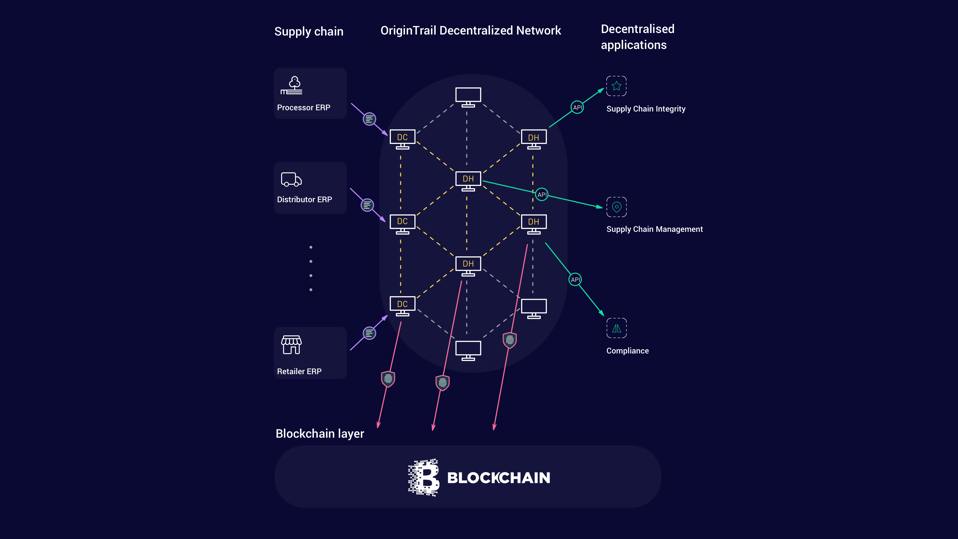
\includegraphics[scale=0.5]{media/origin_trail_network.jpg}
\caption[Overview of the OriginTrail network]{Overview of the OriginTrail network. Available in \cite{OriginTrailTechno}}
\label{fig:origintrail_network}
\end{figure}

\subsubsection{Relevance and Applicability}
This solution specializes more in the tracking of the goods, especially so that the public can know where their products are coming from, as well as the companies. This allows for higher integrity and authenticity of the products. A good example of a use case is in situations where a bad product is detected and batch recalls need to be made. With this tracking, a specific batch can be identified and removed, whereas without the tracking, product providers as well as the product buyers would have to get rid of substantially higher amounts of that product, leading to a loss of revenue.

Though it is a more specialized solution, it is important not to ignore the aspect it focuses on. This can be one of the easiest methods to save money by integrating the supply chain with the blockchain.


\subsection{Ambrosus}
Ambrosus focuses on tracking the quality of the goods transported during shipments, specializing in the food and pharmaceutical industries. Not only does it track shipments throughout the entire supply chain lifecycle, it also uses the Internet-of-Things (IoT), through sensors, to communicate quality metrics of the products in real-time to the blockchain. 

The enterprises can then query this data and retrieve it immediately to their own databases, effectively achieving a better quality assurance. It is also provides enforceable proof of the quality or, if otherwise, the lack of it.

Like OriginTrail, Ambrosus also has its own protocol, called AMB-NET, which hosts smart-contracts and comunicates with the Ethereum blockchain.

\subsubsection{Relevance and Applicability}
This is another project with a more narrow scope, specializing in the tracking of the quality by using IoT. It is something that the other projects are not implementing, but it is important nonetheless. To some industries, it is even more important than any other feature, which makes quality-tracking a \textbf{must} in a supply chain management blockchain project.

%TODO: TALK ABOUT MODUM.IO

\subsection{IBM and Maersk's Demo}
IBM, together with Maersk, just recently launched an innovative project which aims to create an open platform, using Hyperledger, for information sharing on a large scale \cite{A.P.MOLLER-MAERSK}.

It is an open platform, which features a shipping information pipeline and paperless trade. It deals mostly with the transportation of goods and automating all the processes associated with it. 

\subsubsection{Relevance and Applicability}

Although it has a similar purpose to the one of this thesis, there have been reports of companies discontent with this platform, since it does not focus on the industry as a whole and ensure common standards. Instead, it is a platform designed to meet IBM and Maersk's expectations. Other than this, there has been very little information about it yet or about any progress made.

%TODO: PUT A REFERENCE HERE FROM WHERE I READ THIS

%\todo{fcorreia: nothing more to say about this? would be interesting to know in which way it compares with your goals and with the other similar applications}
%It was just announced and they have no articles explaining it yet...

\section{Designing a Blockchain-based Supply Chain}
%CHECK https://modum.io/system/

Blockchain is not always a one-size-fits-all solution, and its use must be carefully tailored to the application in question and to the specific requirements. This section describes some important points of focus to have in mind when making decisions for the design of a blockchain based supply chain.

\subsection{Integration Models}
\paragraph{Point-to-point} Business-to-Business (B2B) Data Interchange - The integration must be designed between each two specific endpoints. Each new connection must be modeled separately. In a large scale, this does not work very well, it is a model that only works under specific cases and requirements, since it requires a customized integration.

\paragraph{One-to-many entities} Hub B2B - A company can develop a connection endpoint to which other companies can connect, as long as they follow the hub's communication standards or use its API. This way, a  single company can establish connections with multiple intermediaries.

\paragraph{Many-to-many entities} Cloud B2B - This model encompasses full integration, where the information can flow freely between businesses. This is the ultimate goal of a public blockchain, but it would require companies the development of interoperability standards, which are, at the moment, lacking. Otherwise, it is the most cost-effect model and the one which can bring about the most benefits as well, given that the companies can develop their services to be integrated with the blockchain.

\subsection{Key Implementation Components and Features}
As seen in the previously mentioned projects, like CargoX, Eximchain and OriginTrail, each of them followed their own purpose and goals, and each of them has a different set of features that allows them to achieve these goals. Similarly, these are some of the key components that a blockchain possesses, and the respective features that must be decided upon:

\paragraph{Information Storage}
The most basic and important feature of a blockchain is the ability to save data, which is then considered immutable, as well as registering any important events. As such, information storage is a must in supply chain. \todo{fcorreia: "is a must" é um pouco informal de mais} It also makes Inventory Management possible (though it's \todo{fcorreia: its} implementation is out of the blockchain's scope), traceability and provenance of products.
      
\paragraph{Ledger and Transactions}
Similarly, allowing for transactions and their recording onto the chain might be important, especially in what accounts for payments between businesses.
  
\paragraph{Smart Contracts}
Finally, smart contracts have the potential to be an important part of SCM. In the applications we described, smart contracts were used to transfer ownership of either data or products through tokens. This is just one of the many possible uses. Other smart contract uses include tracking items by their location or condition, automatically updating the status on the blockchain and reacting to any important events by notifying the organization responsible for the items. Another possible functionality is the automation of payments upon delivery. In the end, smart contracts allow for virtually any application, since they are code, programs being run on the blockchain, and so, they are one of the components of blockchain with the most potential for new and innovative features to be developed upon.
        
%\todo{fcorreia: Something that could be fun to have in this section is a diagram depicting the different concerns that you have to consider and how these different concerns affect each other. For an example, take a look at the diagram in page 3 of this paper: \url{http://blog.invisivel.net/wp-content/papercite-data/pdf/ferreira_core_2010.pdf}}


